\documentclass{slide}

\title{Pipeline Architecture}
\subtitle{CSSE6400}
\author{Brae Webb}
\date{The Future}

\usepackage{languages}

\usepackage{tikz}
\usetikzlibrary{positioning}
\usetikzlibrary{arrows}
\usetikzlibrary{fit}

\begin{document}

\maketitle

\questionanswer{Can you name a \highlight{pipeline archiecture}?}{How about \highlight{bash}?}

\begin{frame}[fragile]
\begin{code}[language=shell,mathescape]{}
$>>$ cat assignment.py | grep "hack" | wc -l \
    | tee code-quality.txt
\end{code}
\end{frame}

\begin{frame}
    \centering
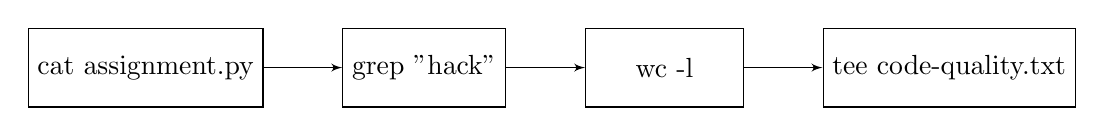
\begin{tikzpicture}[>=latex']
    \tikzset{block/.style= {draw, rectangle, align=center,minimum width=2cm,minimum height=1cm},}

    \node [block] (input) {cat assignment.py};
    \node [block, right =1cm of input] (grep) {grep "hack"};
    \node [block, right =1cm of grep] (wc) {wc -l};
    \node [block, right =1cm of wc] (tee) {tee code-quality.txt};

    \path[draw,->]
                (input) edge (grep)
                (grep) edge (wc)
                (wc) edge (tee)
                ;
\end{tikzpicture}
\end{frame}

\begin{frame}[c]

\only<1->{{\large\par\bigskip
\begin{center}
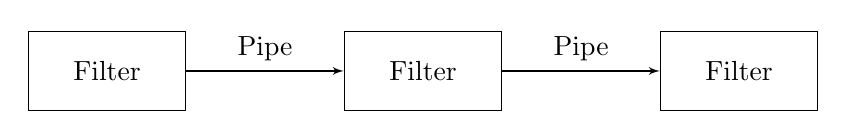
\begin{tikzpicture}[>=latex']
    \tikzset{block/.style= {draw, rectangle, align=center,minimum width=2cm,minimum height=1cm},}

    \node [block] (filter1) {Filter};
    \node [block, right =2cm of filter1] (filter2) {Filter};
    \node [block, right =2cm of filter2] (filter3) {Filter};

    \path[draw,->]
                (filter1) edge node[above] {Pipe} (filter2)
                (filter2) edge node[above] {Pipe} (filter3)
                ;
\end{tikzpicture}
\end{center}
}
}

\only<2->{
    \par\bigskip{\normalsize\color{primary}Filters}

    \huge Modular software components
}

\only<3->{
    \par\bigskip{\normalsize\color{primary}Pipes}

    \huge The flow of data between filters
}
\end{frame}

\begin{frame}
\begin{minipage}{0.45\textwidth}
\only<1->{
    \par\bigskip{\normalsize\color{primary}Producers}

    \huge Source of data.
}

\only<2->{
    \par\bigskip{\normalsize\color{primary}Transformers}

    \huge Transform data.
}
\end{minipage}
\begin{minipage}{0.45\textwidth}
\only<3->{
    \par\bigskip{\normalsize\color{primary}Testers}

    \huge Filter data.
}

\only<4->{
    \par\bigskip{\normalsize\color{primary}Consumers}

    \huge Target for results.
}
\end{minipage}
\end{frame}

\point[Exercise]{Label the bash pipeline.}

\begin{frame}
\centering
\begin{tikzpicture}[>=latex']
    \tikzset{block/.style= {draw, rectangle, align=center,minimum width=2cm,minimum height=1cm},}

    \node [block,label=\only<2->{\only<2>{\color{focus}}Producer}] (input) {cat assignment.py};
    \node [block,label=\only<3->{\only<3>{\color{focus}}Tester}, right =1cm of input] (grep) {grep "hack"};
    \node [block,label=\only<4->{\only<4>{\color{focus}}Transformer}, right =1cm of grep] (wc) {wc -l};
    \node [block,label=\only<5->{\only<5>{\color{focus}}Consumer}, right =1cm of wc] (tee) {tee code-quality.txt};

    \path[draw,->]
                (input) edge (grep)
                (grep) edge (wc)
                (wc) edge (tee)
                ;
\end{tikzpicture}
\end{frame}

\question{Does this seem familiar?}

\point[Poll]{Who has done \highlight{functional programming}?}

\begin{frame}[fragile]
\begin{code}[language=lambda]{}
let sum = reduce 
            (lambda total value -> total + value) 
            (map (lambda seq -> size seq) xs)
            0
\end{code}
\end{frame}

\begin{frame}[fragile]
\begin{code}[language=lambda]{}
let sum = reduce + (map size xs) 0
\end{code}
\end{frame}

\begin{frame}[fragile]
\large
\begin{defn}[$map$]
\begin{code}[language=lambda]{}
map : (type$_1$ -> type$_2$) -> type$_1 Seq$ -> type$_2 Seq$
map $f$ $xs$
\end{code}
\end{defn}
\end{frame}

\begin{frame}[fragile]
\large
\begin{defn}[$reduce$]
\begin{code}[language=lambda]{}
reduce : (type$_1$ -> type$_1$ -> type$_1$) -> type$_1 Seq$ -> type$_1$ -> type$_1 Seq$
reduce $f$ $xs$ $initial$
\end{code}
\end{defn}
\end{frame}

\questionanswer{What's the advantage of the map reduce pattern?}{Parallelism \cite{mapreduce}}

\question{Using pipeline terminology, what filters do the \highlight{map} and \highlight{reduce} operators correspond to?}

\references{articles,books}

\end{document}